% Chapter 2
\chapter{The \lhcb Detector}
\label{lhcb_detector}

\begin{itemize}
  \item Maybe mention charm production. And recently also with rare kaon physics.
\end{itemize}

The \lhcb experiment is an international collaboration located at the {\it European Organization for Nuclear Research}, \cern.
There are four major experiments there; Two of them, \atlas and \cms, serve as a general purpose experiments whereas the other
two \alice and \lhcb, are dedecated to {\it heavy ion} and {\it flavour} physics respectively\footnote{Flavour physics is  defined in and heavy ion in thsi sitation.}.
{\color{red} citation of the experiments}. All of the experiments aim at detecting and recording as many as posible high energy
particle collisions, which are provided by the \lhc acclerator. The last is the world's most powerful particle accelerating
machine built so far. The \lhc machine accelerates and stores two beams of protons. It is also capable of acceprating
and coliding heavy ion beams, \eg led, thus serving the physics program of the \alice experiment.
In both cases beam storage is achieved by magnetically forcing them to follow an eliptical trajectory.
The two beam trajectories are designed such that they colide with each other at four specific points, see \figref{}.
The \lhc accelerator as well as the four above mentioned experiments are located located about $100\m$ udnerground,
to protect human population from radiation. The complexity and techinical dificulties required to build, run and maintain
all these machines is a remarkable achievement of human claboration.

As mentioned above the \lhcb experiment is dedeicateed to study the kind of physics described in \secref{}.
The design of the \lhcb detector is the result of an optimization for this particular kind of physics.
Specifically, the experiment focuses in detecting \B mesons, explained in \secref{}. The latter type of
meson contains a \bquark quark which originates from a proton-proton colision. In \figref{} it can be seen
that \bquark quarks produced in such a colision, cluster mainly along the proton beam axis. In other words
roughly $50\%$ of the \bquark quarks {\it fly} inside a region of $\sim 45\circ$ solid angle along the beam axis.
This region is also called {\it forward} region. {\color{red} mention the lhcb acceptance  which is half of the b qurks}The design of \lhcb detector, shown in \figref{}, is such that
it exploits this special production feature of \bquark quarks. Implying that a $4\pi$ detector geometry like the
rest of the \lhc experiments, where the center of colision is sourounded by layers of detectors, is not necessary.
This allows for increased purity of the recorded \B mesons at the expence of a limited physics program compared
to the rest of the \lhcb experiments.

The full \lhcb detector specifications, designs and performance are described in \cite{jnst}.
The aproach of the current chapter is to briefly address the function and perfromance of each detector component,
throughout \secref{det_tracking} - \secref{det_calo}. Emphasis, is given to these sub-detectors that are relevant
to the analysis performed in \chapref{Data_Analysis} as well as to the trigger system which is a partial hardware
and software implementation. The special software based techninique to distinguish between \B and $\Bbar$ decays, called
{\it flavour tagging}, is described in \secref{}.

\begin{figure}[t]
  \centering
  \includegraphics[width=\textwidth]{Figures/Chapter2/detector_cross_cmyk}
  \caption{Crossesctional view of the \lhcb detector.}
  \label{lhcb_detector_cross_section}
\end{figure}

\begin{figure}[t]
  \centering
  \includegraphics[width=0.7\textwidth]{Figures/Chapter2/08_rad_acc_scheme_right}
  \caption{bb quark pair production.}
  \label{bb_roduction_angles}
\end{figure}



\section{Tracking System}
\label{det_tracking}

The tracking system is used for

Need to mention-describe:
\begin{itemize}
  \item reconstruction
  \item types of tracks
  \item long track reco efficiency
  \item momentum resolution of the whole tracking system, (this drives ang. res of ana chap)
  \item proper time resolution, see plot
\end{itemize}

\begin{figure}[t]
  \centering
  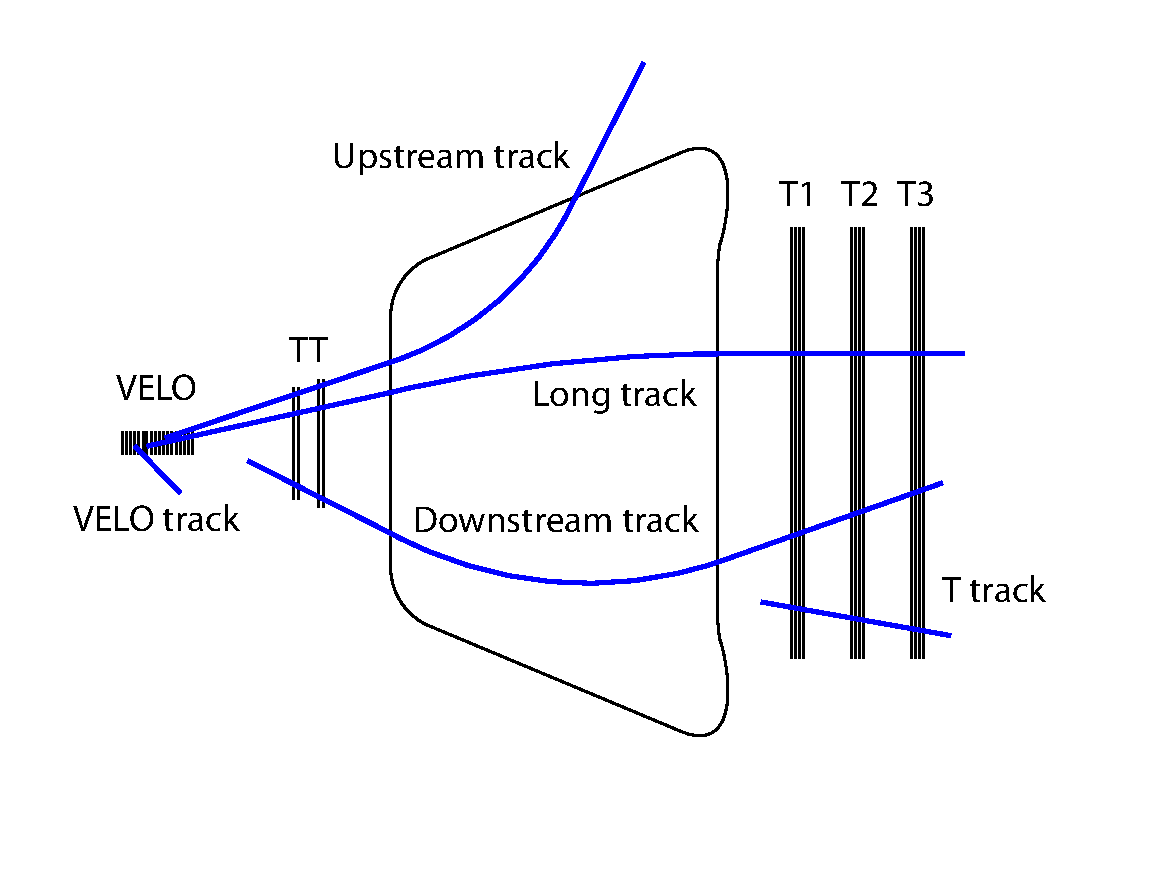
\includegraphics[width=0.7\textwidth]{Figures/Chapter2/trackTypesRunIAndII}
  \caption{\lhcb track types.}
  \label{track_types}
\end{figure}

\subsection{VeLo}
the velo track reco eff is more thatn 90 percent

\subsection{TT}
The veloTT track reco eff is more thatn 95 percent
The ghost rate is improved by 20 percent totaling to 95 percent or something

\subsection{OT}

\begin{figure}[t]
  \centering
  \includegraphics[width=0.7\textwidth]{Figures/Chapter2/final_decay_time_res_plot1}
  \caption{\lhcb proper type resolution.}
  \label{track_types}
\end{figure}


\section{Particle Identification}
Pid system supresses backgrounds by a lot.
Used in every analysis.
You have those rich detecotrs and the performance is blah.

\begin{itemize}
  \item Electron ID  90 % for ~ 5 % e→h mis-id probability
  \item Kaon ID 95 % for ~ 5 % π→K mis-id probability
  \item Muon ID 97 % for 1-3 % π→μ mis-id probability
\end{itemize}

\section{Muon system}
The muon system has a variant granularity because blah.
The resolution varies from this to that
The efficiency is this

\section{Calorimeters}
\label{det_calo}
Calorimeters provide energy information for neutrals.
Sambling calorimeters, ecal and hcal.
They also stop hadrons, whereas mip muons penetrate led.
Information from calorimeters are not used

\section{The trigger system}
\label{det_trigger}

Need to mention-describe:
\begin{itemize}
  \item The trigger is responsible for .....
  \item It is consits of L0 Hlt1 hlt2
  \item mention defral triggered events
  \item The output is organised in 4 L0 streams.
  \item Hlt1 and hlt2 is organised in lines.
  \item It is intreasting to see the improvement of the trigger from run one to run two.
  \item Show the organisation of the performance of the muon lines.
\end{itemize}

\begin{figure}[t]
  \centering
  \includegraphics[width=0.4\textwidth]{Figures/Chapter2/LHCb_Trigger_RunIAlgDetail_May2015}
  \includegraphics[width=0.4\textwidth]{Figures/Chapter2/LHCb_Trigger_RunII_May2015}
  \caption{\runone trigger scheam.}
  \label{run_one_trigger}
\end{figure}


\section{Favour Tagging}
\label{det_tagging}

\section{The \BJpsiKst Decay in \lhcb}
\label{BspsiKst_at_lhcb}
\begin{itemize}
  \item Production of \Bs mesons (how many),
  \item Estimate of the expected yield
  \item Event display
  \item Maybe define observables
\end{itemize}
